\section{Task 5: what to build, where, and in what order}\label{sec:q5}

\subsection{From hazard to a decision variable}

A construction plan is an allocation of money across measures, so the model must price risk. We use a three-day event scale throughout, because that is the scale at which the two storms of Section~\ref{sec:q4} caused damage.

\textbf{Hazard.} For each city, annual maximum three-day rainfall $X$ is fitted with a GEV by L-moments over 1961--2020. The design depth for a $T$-year standard is $\mathrm{RL}_{3d}(T)$; for Zhengzhou it is 102.9\,mm at $T=2$, 162.3\,mm at $T=10$ and 207.2\,mm at $T=50$, against an observed 2021 value of 313.4\,mm (station) and 449\,mm (official).

Two accounting conventions coexist here and answer different questions. Task~1 asks how much water arrives in the peak window and how long the network needs to clear it; Task~5 asks what a year of rainfall costs, so it routes the 72-hour total through the same curve-number model and prices the resulting volume against capacity. The Task~1 peak-hour excess of $1.4\times10^{8}$\,m$^3$ and the Task~5 event budget of $3.50\times10^{8}$\,m$^3$ are therefore not interchangeable.

\textbf{Capacity and damage.} Capacity is $C=\mathrm{RL}_{3d}(T)+S_{\text{sto}}$, the design rainfall depth plus the depth equivalent of distributed storage $S_{\text{sto}}$. Both the hazard and the overflow are measured in \emph{runoff} space: the three-day total $X$ is routed through the SCS-CN curve, whose retention is $S_{\text{ret}}=25400/\mathrm{CN}-254$, to give $Q(X)$, and overflow is $O=(Q(X)-C)^+$. Damage is carried by overflow \emph{volume}, not depth, because a city of 230\,km$^2$ cannot lose the same absolute amount as one of 1\,180\,km$^2$ at the same depth. Writing $V=O\cdot A$ and $V_{\text{ref}}=O_{\text{ref}}\cdot A_{\text{ZZ}}$, the loss law is
\[
D(X)=D_{2021}\left(\frac{V}{V_{\text{ref}}}\right)^{1.5}
       =D_{2021}\left(\frac{A}{A_{\text{ZZ}}}\right)^{1.5}
        \left(\frac{O}{O_{\text{ref}}}\right)^{1.5},
\]
so that $D(O_{\text{ref}})=D_{2021}$ for Zhengzhou by construction, and any other city is scaled by its own built-up area. For Zhengzhou, $Q(449)=399.4$\,mm against a two-year capacity of 102.9\,mm gives $O_{\text{ref}}=296.4$\,mm, equivalent to $3.50\times10^{8}$\,m$^3$ of excess water and a loss density of 116.9 CNY per m$^3$. The convexity encodes the observed fact that damage grows faster than flooded volume once underground space and critical infrastructure begin to fail; the exponent is an assumption, and Section~\ref{sec:eval} varies it between 1.2 and 1.8.

\textbf{Cost.} Three measures are priced: (i) conveyance capacity, 0.85 million CNY per millimetre of added design depth per km$^2$, i.e.\ one billion CNY for one millimetre over Zhengzhou's built-up area (a unit that absorbs pipe diameter, pumping and land acquisition); (ii) distributed storage, 800 CNY per m$^3$ of volume; (iii) green source control, 150 million CNY per km$^2$ for full coverage, with a curve-number reduction of up to 40 points at 30\% coverage. Expected annual damage is the sample mean of $D$ over the 1961--2020 annual maxima (no tail extrapolation beyond the observed range), and the risk term is the mean of the upper 5\% of the same sample. The death term uses a value of a statistical life of 5 million CNY and a death elasticity of 1.5 with respect to overflow. Costs and benefits are discounted at 4\% over a 30-year horizon with 2\% annual operation and maintenance, and risk is priced with a 0.5 weight on the 95\% conditional value-at-risk, so a plan that only looks good on average is penalised. Each unit cost is a planning-grade assumption rather than a tendered price; Section~\ref{sec:eval} reports the ranges over which the ranking is stable.

The decision is a triple $(T,S_{\text{sto}},g)$ over $T\in\{2,3,5,10,20,50,100\}$, $S_{\text{sto}}\in\{0,5,10,20,40,80\}$\,mm and $g\in\{0,0.15,0.30\}$, evaluated for Zhengzhou, Guangzhou and Haikou. The benefit--cost ratio is reported both economically (avoided damage only) and socially (avoided damage plus avoided deaths).

\subsection{Uniform upgrading does not pay anywhere}

Table~\ref{tab:q5base} gives the baseline risk of the three cities under the current two-year standard. Guangzhou carries the largest expected annual damage (11.3 hundred million CNY), because it combines a high hazard with a 1\,400\,km$^2$ exposure; Zhengzhou's is the lowest (2.46), a direct consequence of its relatively benign three-day climatology.

\begin{table}[H]
\centering
\caption{Baseline risk under the current two-year design standard. EAD is expected annual damage; deaths are expected annual deaths.}
\label{tab:q5base}
\small
\begin{tabular}{lrrrr}
\toprule
City & RL$_{3d}$(2) (mm) & RL$_{3d}$(50) (mm) & EAD ($10^8$ CNY) & Expected deaths\\
\midrule
Zhengzhou & 102.9 & 207.2 & 2.46 & 2.29\\
Guangzhou & 166.4 & 344.5 & 11.31 & 12.05\\
Haikou & 201.6 & 574.7 & 3.12 & 7.67\\
\bottomrule
\end{tabular}
\end{table}

Optimising the 378-point grid produces a blunt result: for all three cities the cost-minimising uniform plan is \emph{no investment at all}. The best uniform ratios are 0.28 (Guangzhou, 5\,mm of storage), 0.18 (Haikou, 5\,mm) and 0.10 (Zhengzhou, 5\,mm); none reaches break-even, and the social objective does not rescue them, because the avoided deaths are too few to close a gap of that size. Only one social plan does better than nothing --- 20\,mm of storage in Guangzhou, cutting expected damage by 38\% for a social ratio of 0.26 --- and it too stays below one.

The reason is arithmetic: one millimetre of design depth over Zhengzhou costs a billion CNY, four times that city's entire expected annual damage, because extreme events are rare while capacity is paid every year. This is not an argument against standards, which also protect against frequent events and the tail beyond the fitted range, but against uniform capacity as the \emph{first} purchase.

\subsection{Targeted protection is where the money works}

Uniform capacity spreads money over area that is rarely flooded, yet the 2021 losses were concentrated in a few square kilometres of underpasses, metro stations and low-lying districts. We therefore add a second decision: protect a fraction $h$ of the city where damage density is $m$ times the average and leave the rest at baseline. Table~\ref{tab:q5sel} reports the benefit--cost ratio for each pair at the optimal storage depth of 5\,mm; the optimum is always the smallest positive increment, because hotspot damage density is high enough that the first increment captures almost all the benefit.

\begin{table}[H]
\centering
\caption{Benefit--cost ratio of targeted protection: fraction $h$ of the city protected, damage density $m$ times the city average, at 5\,mm of local storage.}
\label{tab:q5sel}
\footnotesize
\setlength{\tabcolsep}{4pt}
\begin{tabular}{lrrrr}
\toprule
City & $h{=}2\%$ & $h{=}5\%$ & $h{=}2\%$ & $h{=}5\%$\\
 & $m{=}10$ & $m{=}10$ & $m{=}20$ & $m{=}20$\\
\midrule
Guangzhou & 2.37 & 1.93 & 4.05 & 2.87\\
Haikou & 1.53 & 1.25 & 2.62 & 1.85\\
Zhengzhou & 0.88 & 0.71 & 1.50 & 1.06\\
\bottomrule
\end{tabular}
\end{table}

Targeted protection is an order of magnitude more efficient than uniform capacity, and it reverses the verdict wherever there is a dense core. Guangzhou, whose best uniform ratio was 0.28, returns 4.05 when the 2\% most exposed area carries twenty times the average damage; Haikou returns 2.62; Zhengzhou, the least exposed of the three, clears break-even only at the two most favourable assumed pairs (1.50 at $h{=}2\%$, $m{=}20$; 1.06 at $h{=}5\%$, $m{=}20$). Across the nine assumed $(h,m)$ pairs and the five positive storage depths, 62 of 135 evaluated combinations clear break-even, and the highest ratio is 4.05 (Figure~\ref{fig:bcr} sets the two menus side by side). The ranking across cities is stable --- Guangzhou first, then Haikou, then Zhengzhou --- which is the opposite of the hazard ranking, because what matters for a hotspot investment is the absolute damage density, and Guangzhou's larger exposure more than offsets Haikou's higher design depth. The ratio itself is driven by the two assumptions of this experiment, but the ordering survives every assumed pair.

\subsection{A risk-constrained stochastic programme}

Menus answer ``which option is cheapest''; a city actually asks ``how much risk may remain''. We therefore restate Task~5 as a scenario-based stochastic programme. The scenarios are the 60 observed annual maximum three-day depths of 1961--2020 with equal weights, so the risk measure uses no tail extrapolation. The decisions are the added conveyance depth $C_{\text{add}}\ge0$ beyond the current two-year design, the storage depth $S_{\text{sto}}\ge0$, and a source-control share $g$. Cost is the annualised capital charge; damage follows the calibrated convex function; risk is the 95\% conditional tail expectation of annual damage, $\mathrm{CVaR}_{95}$, the mean of the worst 5\% of the 60 scenarios. The programme is

\begin{equation}
\min_{C_{\text{add}},S_{\text{sto}},g}\ \text{annual cost}\quad\text{s.t.}\quad \mathrm{CVaR}_{95}(C_{\text{add}},S_{\text{sto}},g)\le B,
\end{equation}

solved exactly on a $2.5$\,mm lattice in $(C_{\text{add}},S_{\text{sto}})$ for each of three source-control levels, and for a ladder of caps $B$ expressed as a fraction of the no-investment risk. The resulting frontier is Figure~\ref{fig:pareto}; the caps are insurance, and the question is whether the premium is worth paying.

\begin{figure}[H]
\centering
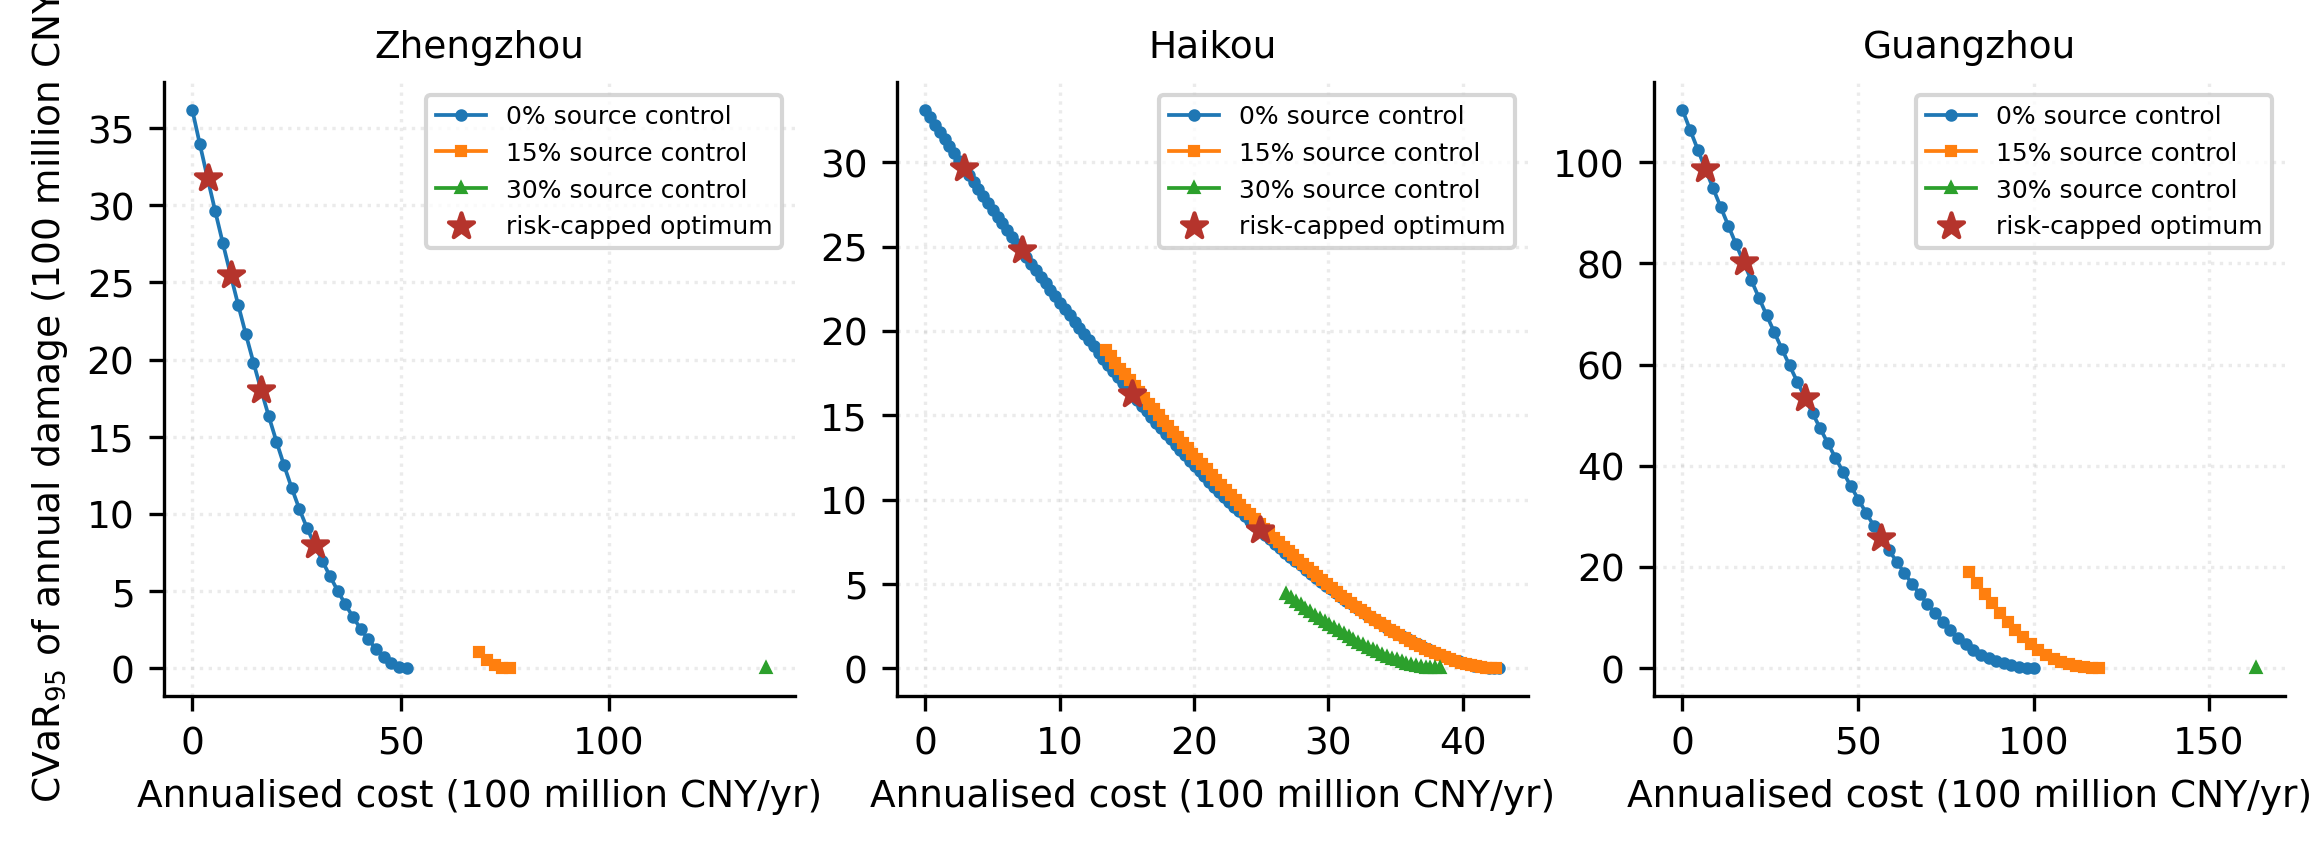
\includegraphics[width=0.36\linewidth]{../02_figures/fig23_q5_pareto.png}
\caption{Annualised cost against $\mathrm{CVaR}_{95}$ of annual damage for the three cities, for three source-control shares; stars mark the cost-minimal design under each risk cap. Lower-left is better and the frontier is the lower envelope.}
\label{fig:pareto}
\end{figure}

Three results follow. First, without a risk cap no city invests: the unconstrained optimum is the status quo everywhere, the same verdict as the uniform menu. Second, a binding cap forces spending, and what it buys differs by city: at 90\%, 50\% and 25\% of baseline risk Zhengzhou buys 5, 22.5 and 40\,mm of storage (ratios 0.10, 0.085, 0.068), Guangzhou 7.5, 40 and 65\,mm of extra conveyance (0.27, 0.21, 0.17), and Haikou 20, 107.5 and 150\,mm of storage (0.17, 0.13, 0.11), the tightest cap adding 22.5\,mm of conveyance, i.e.\ a three-year equivalent standard, rather than source control. Third, every ratio here is below one while every hotspot ratio above is above one: \emph{a risk cap is a constraint, not an investment}. A city that must meet a residual-risk target should meet it at least cost, and the least-cost instrument is the hotspot, which this programme cannot buy because its decision variable is a city-wide depth.

\subsection{A three-speed construction plan}

\textbf{Speed 1: protect the hotspots (0--5 years).} Identify the 2--5\% of each city where damage density is at least ten times the average (underpasses, metro portals, underground car parks, hospitals, power substations) and protect exactly those with local storage, raised entrances, sealed shafts and pumped drainage. The ratio is 1.0--4.1 across the assumed pairs, the measure is reversible and fast, and closure protocols for underground space should be written into the operating licence, because the Zhengzhou failure was as much a decision failure as an engineering one.

\textbf{Speed 2: source control where it is cheap (5--15 years).} Green roofs, permeable pavement and detention ponds reduce the curve number and the runoff volume, at 150 million CNY per km$^2$ of full coverage. Our grid shows that 15--30\% coverage never pays on its own; it also delivers amenity and heat benefits the model does not monetise, so it belongs where land is cheap and redevelopment is already happening.

\textbf{Speed 3: conveyance capacity only where exposure is extreme (15--30 years).} Deep tunnels and large pumping stations cost a billion CNY per millimetre of design depth over a city like Zhengzhou; they pay only under a binding risk cap, and even there storage is the cheaper instrument. For most cities the money is better spent on the first two speeds plus non-structural measures.

\textbf{Cross-cutting: measure the right variable.} Section~\ref{sec:q3} showed that a daily-index screen misses a Zhengzhou-type disaster entirely. Every city should therefore archive sub-hourly precipitation and publish design storms at both a three-day and an hourly duration. The current Chinese standard (GB\,50014-2021 \cite{gb50014}, with GB\,55027-2022 \cite{gb55027}) already defines the storm-water system as source reduction, conveyance and detention plus non-structural measures, and sets design return periods of 1--3 years for ordinary, 3--5 for important and 10 for especially important areas; our results say that this ladder is reasonable for conveyance, but that the binding constraint on catastrophic loss is the unprotected hotspot, not the pipe diameter.

\textbf{Staged budget.} For Guangzhou, protecting 2\% of the 1\,400\,km$^2$ area with 5\,mm of local storage means $1.4\times10^{5}$\,m$^3$, about 112 million CNY at the unit cost used here; with sealed entrances and operating procedures the first phase stays well below half a billion CNY, several times less than one millimetre of city-wide capacity over the same area (1.19 billion CNY), and it returns 4.05 times its cost in avoided damage before deaths are counted.
